\documentclass[11pt,a4paper,openany,leqno]{article}

\textwidth=160mm \textheight=260mm \hoffset=-18mm \voffset=-30mm
\setcounter{page}{1}
			\usepackage[magyar]{babel}
			\usepackage[utf8]{inputenc}
			\usepackage[T1]{fontenc}
			\usepackage{indentfirst}
			\usepackage{amsmath,esint}
			\usepackage{amssymb}
%			\usepackage{eufrak}
			\usepackage{psfrag}
			\usepackage{tabularx}
			\usepackage{graphicx}
			\usepackage{wrapfig}	
			\usepackage{hyperref}
			\usepackage{multicol}	
									
			\frenchspacing
			\allowhyphens

\tolerance=2000
\hbadness=2000
\vbadness=10000
\overfullrule=0pt




\begin{document}
\section{Dielektrikumok}
\subsection{Elméleti Fizikai Példatár II./ 3.2. feladat}



Egy sík a teret két részre osztja. A felső térrész deilektromos állandója $\varepsilon_1$, az alsóé $\varepsilon_2$. A felső térrészben az elválasztó síktól h távolságra, a felülettel párhuzamosan végtelen hosszúnak tekinthető vonaltöltés helyezkedik el.

\medskip
$a)$ Határozzuk meg a potenciált!

\medskip
$b)$ Mekkora erő hat a töltés L hosszúságú szakaszára?

\begin{flushright} {Feladatot kidolgozta: {\it Z2R8XS}} \end{flushright}

\vspace{0.5cm}

\textbf{Megoldás}


A feladat megoldásához szükséges megemlíteni egy jelenséget. Ha két egymással érintkező dielektrikumot elektromos erőtérbe helyezünk, az érintkező felület töltötté válik. Ez annak köszönhető, hogy a kétféle anyagban eltérő a relatív permittivitás, vagyis másképp polarizálódnak, ezért a határfelületen ellentétes előjelű és különböző nagyságú polarizációs töltések lesznek. \\ \indent
Egy vonaltöltés által létre hozott elektromos tér a következőképp néz ki:
$$E = \frac{\eta}{2 \pi \varepsilon_0 \varepsilon_r} \frac{1}{r} $$
\indent
Itt $r$ a vonaltöltés által kielölt egyenestől vett távoltságot jelenti. Az egyenesre merőleges síkban mindig radiális irányú. A térerősség vektornak nincs ezzel az egyenessel párhuzamos komponense.
\\ \indent
A tükörtöltés módszere alkalmazható. \\ \indent
\begin{figure}[h!]
\centering
  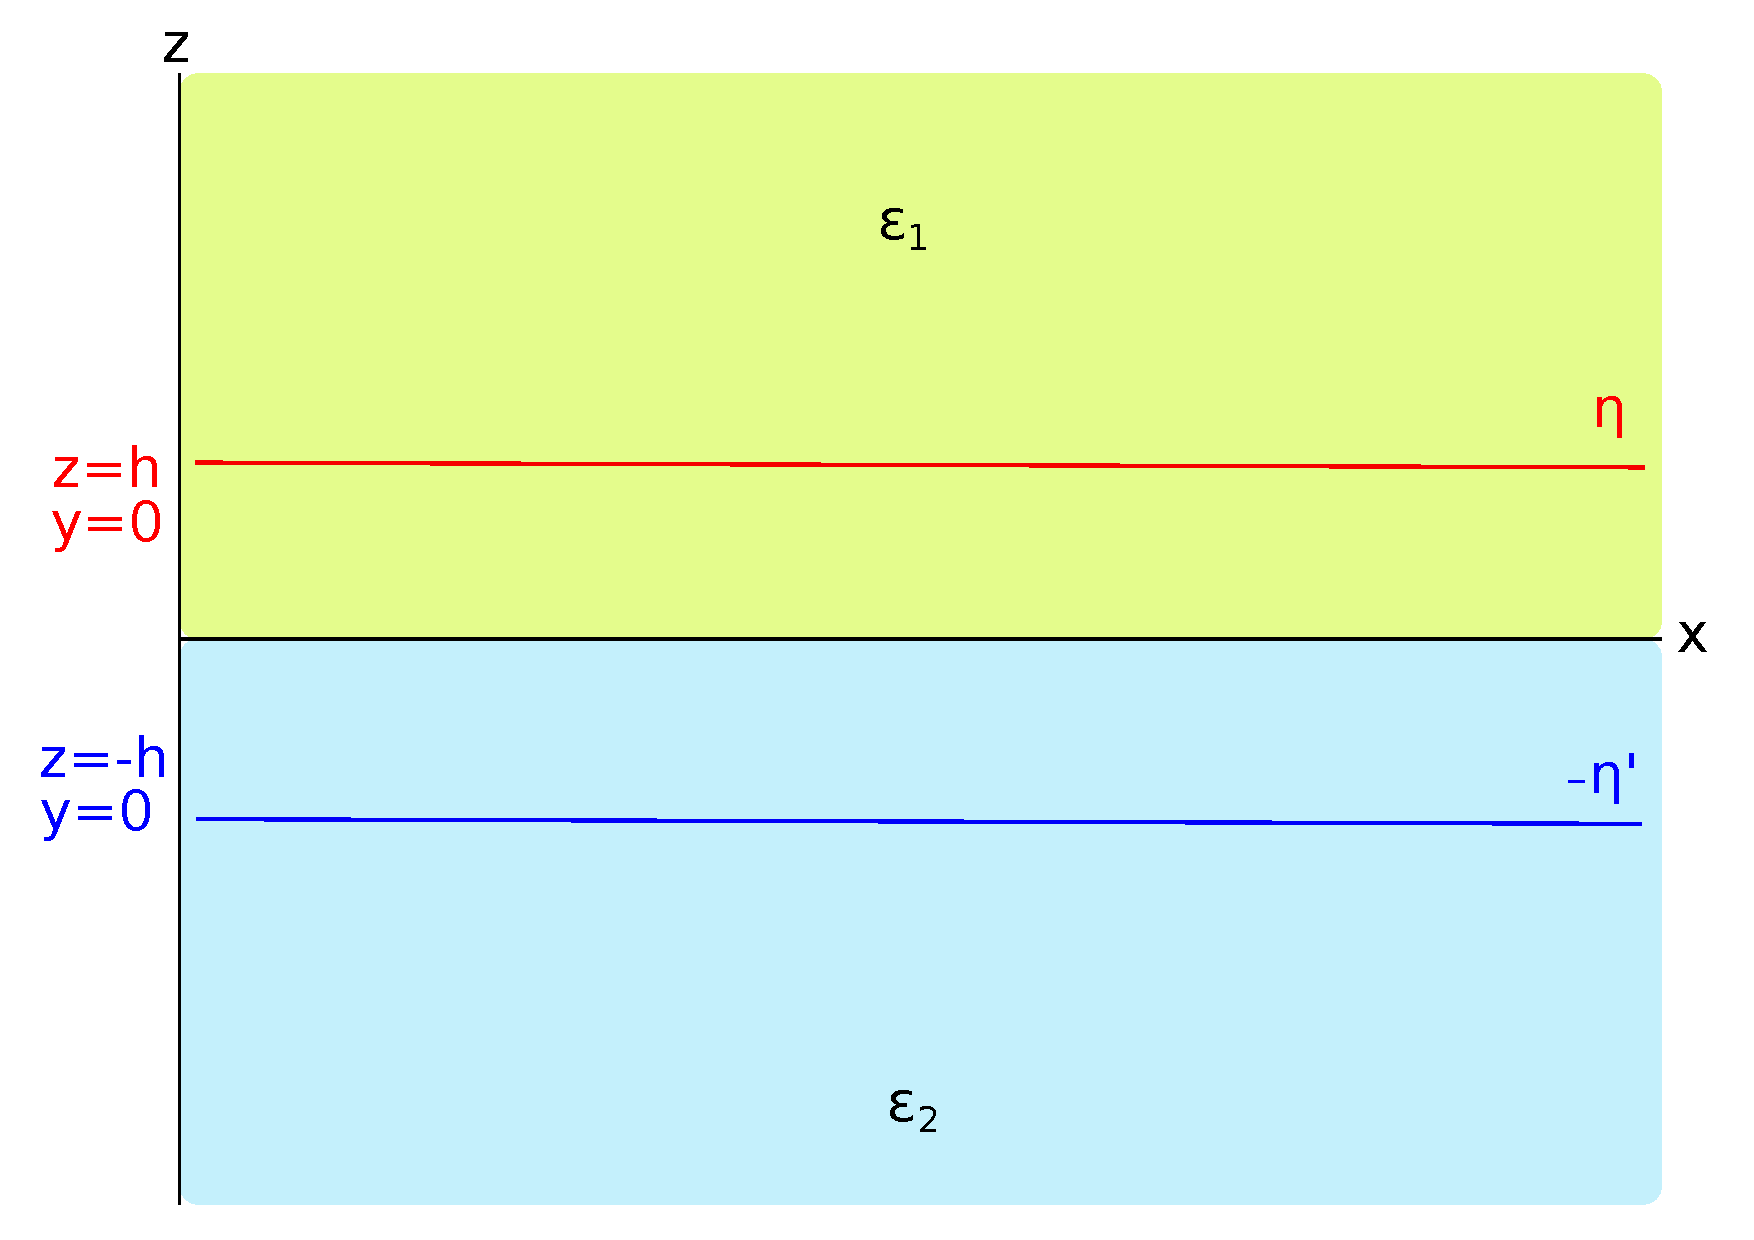
\includegraphics[width=120mm,scale=0.5]{beadando1_1.pdf}
  \caption{A felső térrész elektromos terének szemléltetése}
  \label{}
\end{figure} \\ \indent
A felső térrészben az elektromos tér úgy néz ki, mintha az eredeti $\eta$ töltéssűrűségű vonaltöltés és egy $\eta'$ töltéssűrűségű vonaltöltés hozta volna létre. Mivel $\Phi(r) = - \nabla \vec{E}(r)$ és a vonaltöltés az $(x,z)$ síkban helyezkedik el : 
$$ \Phi_1 = -\frac{\eta}{4 \pi \varepsilon_0 \varepsilon_1} ln(r^2) + \frac{\eta'}{4 \pi \varepsilon_0 \varepsilon_1} ln(r'^2) $$
$$\Phi_1 = -\frac{\eta}{4 \pi \varepsilon_0 \varepsilon_1} ln(y^2 + (z-h)^2) + \frac{\eta'}{4 \pi \varepsilon_0 \varepsilon_1} ln(y^2 + (z+h)^2)$$
\indent
Az alsó térrészben az elektromos térerősség olyan, mintha egy vonaltöltés hozta volna volna létre, melynek $\eta"$ töltéssűrűsége van. Ez úgy magyarázható, hogy az eredeti vonaltöltés által létrehozott tér gyengítve van, mivel a két dielektrikum közt lévő határfelületen megjelent töltések árnyékolják.\\
\begin{figure}[h!]
\centering
  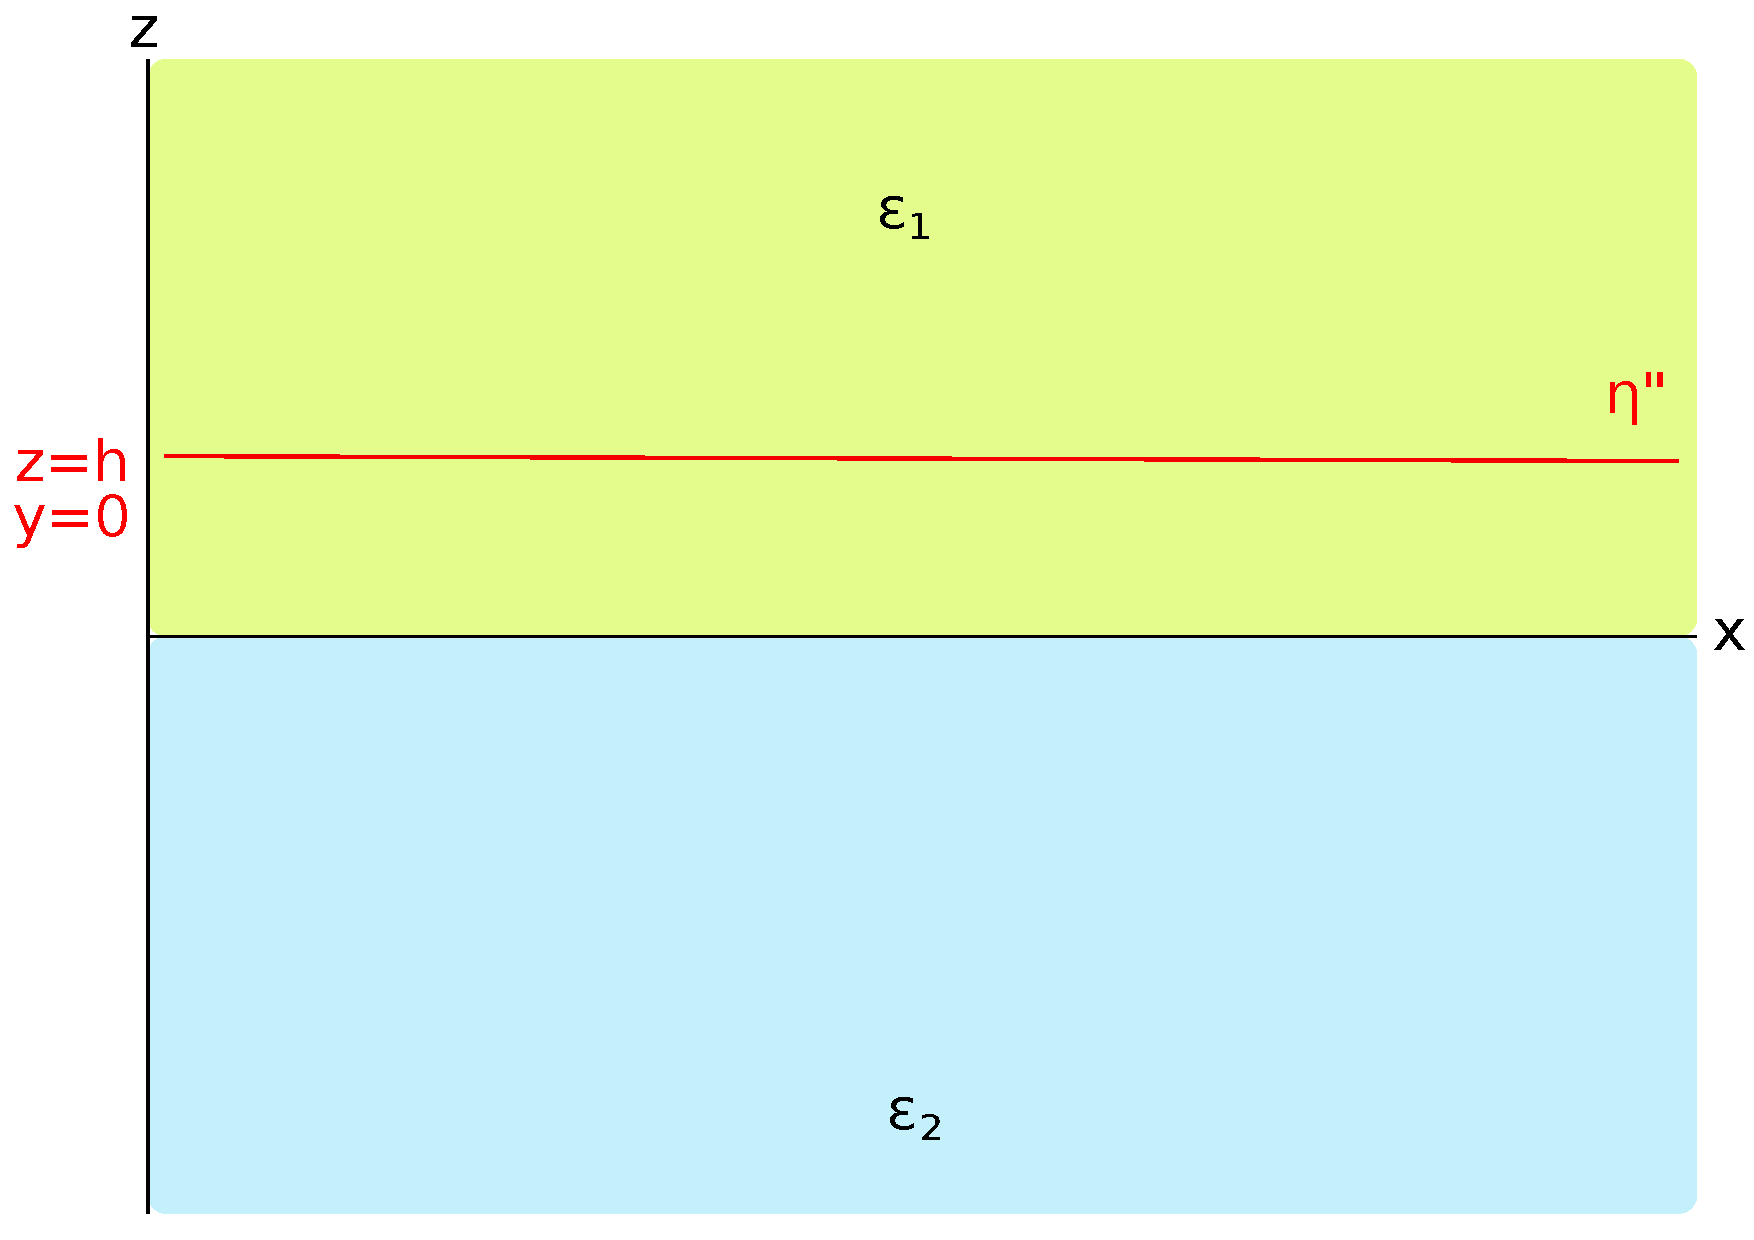
\includegraphics[width=120mm,scale=0.5]{beadando1_2.pdf}
  \caption{Az alsó térrész elektromos terének szemléltetése}
  \label{}
\end{figure} \\ \indent
\indent
Hasonló módon felírható:
$$ \Phi_2 = -\frac{\eta"}{4 \pi \varepsilon_0 \varepsilon_2} ln(r"^2) $$
$$ \Phi_2 = -\frac{\eta"}{4 \pi \varepsilon_0 \varepsilon_2} ln(y^2 + (z-h)^2) $$
\indent
A töltéssűrűségek meghatározhatóak a határfeltételek egyenletei alapján. Az első határfetétel, hogy a két elektromos tér felülettel párhuzamos komponensei (tangenciális) megegyeznek a határfelületen. Bevezethető az elektromos térerősség vektor "beesési szöge", ami $\phi$ jelölés alatt fog futni. Mivel az első térben a két vonaltöltés sűrűsége ellentétes előjelű, ezért tangeciális komponenseik kivonódnak.
$$ (\vec{E_1})_t = (\vec{E_2})_t $$
$$ (\frac{\eta}{2 \pi \varepsilon_0 \varepsilon_1} \frac{1}{r} - \frac{\eta'}{2 \pi \varepsilon_0 \varepsilon_1} \frac{1}{r'}) sin(\phi) = \frac{\eta"}{2 \pi \varepsilon_0 \varepsilon_2} \frac{1}{r"} sin(\phi)$$
$$ \frac{\eta}{\varepsilon_1} \frac{1}{r} - \frac{\eta'}{\varepsilon_1} \frac{1}{r'} = \frac{\eta"}{\varepsilon_2} \frac{1}{r"}$$
\indent
Mivel a határfelületen vagyunk, ezért $r = r' = r" = \sqrt{y^2 + h^2}$, vagyis:
$$ \frac{\eta}{\varepsilon_1} - \frac{\eta'}{\varepsilon_1} = \frac{\eta"}{\varepsilon_2}$$
\indent
A másik határfeltétel, hogy a két elektromos eltolás térnek felületre merőleges (normális) komponensei megegyeznek a határfelületen. Mivel az első térben a két vonaltöltés sűrűsége ellentétes előjelű, ezért normális komponenseik összeadódnak.
$$ (\vec{D_1})_n = (\vec{D_2})_n $$
$$ \varepsilon_1 (\vec{E_1})_t = \varepsilon_2 (\vec{E_2})_t $$
$$ \varepsilon_1 (\frac{\eta}{2 \pi \varepsilon_0 \varepsilon_1} \frac{1}{r} + \frac{\eta'}{2 \pi \varepsilon_0 \varepsilon_1} \frac{1}{r'}) cos(\phi) = \varepsilon_2 \frac{\eta"}{2 \pi \varepsilon_0 \varepsilon_2} \frac{1}{r"} cos(\phi)$$
$$ \eta + \eta' = \eta" $$
\medskip
$$ (\eta - \eta')\varepsilon_2 = (\eta + \eta') \varepsilon_1 $$
$$ \eta' = \frac{\varepsilon_2 - \varepsilon_1}{\varepsilon_1 + \varepsilon_2} \eta $$
$$ \eta" = \frac{2\varepsilon_2}{\varepsilon_1 + \varepsilon_2} \eta $$
\indent
Egy $L$ hosszúságú darabon $L\eta$ töltés van. Mivel az eredeti vonaltöltés önmagával nem hat kölcsön:
$$ F = - \frac{\eta'\eta L}{2 \pi \varepsilon_0 \varepsilon_1}\frac{1}{\sqrt{y^2 + (z+h)^2}} $$
\indent
A vonaltöltés elhelyezkedése : $z = h$, $y = 0$.
$$ F = -\frac{\eta'\eta L}{2 \pi \varepsilon_0 \varepsilon_1}\frac{1}{2h} $$
$$ F = -\frac{\eta'\eta L}{4 \pi \varepsilon_0 \varepsilon_1 h} $$
$$ F = \frac{\eta^2 L}{4 \pi \varepsilon_0 \varepsilon_1 h} \frac{\varepsilon_1 - \varepsilon_2}{\varepsilon_1 + \varepsilon_2}$$






\end{document}